
\section{Quantile-based classifiers for multivariate data}
\label{sec:multivariate-classifier}

Having presented and characterized the (inherently univariate) quantile
classifier, our goal then is to construct a classification method for data with
multivariate features based upon the quantile classifier.  We begin by extending
some of the notation from the previous section to the multivariate setting.

First, consider two populations $\Pi_0$ and $\Pi_1$ with corresponding
distribution functions $F_0$ and $F_1$ each on $\mathbb{R}^{p}$, and further let
$F_{0j}$ and $F_{1j}$ denote the marginal distribution functions for the $j$-th
variable with respect to $F_0$ and $F_1$, $j = 1, \dots, p$.  Then we denote the
quantile distance of a point $z \in \mathbb{R}$ to the $\theta$-th quantile of a
population's $j$-th component as
\begin{equation}
  \label{eq:multivariate-phi}
  \Phi_{ij}(z, \theta) =
  \rho_{\theta}\Big(z - F_{ij}^{-1}(\theta) \Big),
  \hspace{5mm} i = 0, 1, \hspace{3mm} j = 1, \dots, p.
\end{equation}
Then the difference of the quantile distances of a point $z$ to the populations'
$\theta$-th quantile of the $j$-th component is defined as
\begin{equation}
  \Lambda_j (z, \theta) = \Phi_{1j}(z, \theta) - \Phi_{0j}(z, \theta),
  \hspace{5mm} j = 1, \dots, p.
\end{equation}
The main idea then of the composite quantile-based classifiers proposed in the
next section is to aggregate the discriminatory information contained in each of
the $\Lambda_j$'s so as to construct a classification method for data with
multivariate features.

\subsection{Composite quantile-based classifiers}
\label{sec:varying-coefficient}

Consider a point $\vec{z} = (z_1, \dots, z_p) \in \mathbb{R}^p$ and quantile
levels $\vec{\theta} = (\theta_1, \dots, \theta_p) \in (0, 1)^p$.  Then the
difference of the quantile distances of the $j$-th component of $\vec{z}$ to the
populations' $\theta_j$-th quantile of the $j$-th component
$\Lambda_j(z_j, \theta_j)$ provides some discriminatory information for the
classification of $\vec{z}$.  In more detail, if $\Lambda_j(z_j, \theta_j)$ is a
large positive value (large relative to the magnitude of the $j$-th component),
then this indicates that $z_j$ is much closer to the $\theta_j$-th quantile of
the $j$-th component of population $\Pi_0$ than it is to the $\theta_j$-th
quantile of the $j$-th component of population $\Pi_1$.  In this event we would
interpret this as being fairly suggestive that $\vec{z}$ is a member of class
$\Pi_0$.  If however, $\Lambda_j(z_j, \theta_j)$ is positive with a small
magnitude, then it is less strongly suggestive that $\vec{z}$ is a member of
class $\Pi_0$.  On the other hand, if $\Lambda_j(z_j, \theta_j)$ is negative,
then this indicates that $z_j$ is closer to the $\theta$-th quantile of the
$j$-th component of population $\Pi_1$ than it is to the $\theta$-th quantile of
the $j$-th component of population $\Pi_0$, and we would interpret this as being
suggestive that $\vec{z}$ is a member of class $\Pi_1$.  Finally, if
$\Lambda_j(z_j, \theta_j)$ has a value of 0, then $z_j$ has an equal quantile
distance to class $\Pi_0$ as to class $\Pi_1$, so we would interpret this as
providing no discriminatory information for the classification of $\vec{z}$.

The question then is how to construct a classification method based on
information obtained from each of the difference of the quantile distances
$\Lambda_j(z_j, \theta_j)$.  Intuitively, we want to classify an observation to
the population for which it has more components that are closer to the
population's component-wise quantiles.  A natural way to incorporate both the
distances and the number of components that an observation is closer to is to
simply sum up the $\Lambda_j(z_j, \theta_j)$'s and see whether this result is
positive (suggesting that the observation belongs to population $\Pi_0$), or
negative (suggesting that the observation belongs to population $\Pi_1$).  This
approach has a few difficulties however.  One potential drawback is that equal
weight is given to each of features.  Naturally, some features may potentially
be more discriminatory and we would like to draw more heavily on these features
for classification purposes, or conversely we would like to draw less heavily on
less discriminatory features.  A second is an issue of scaling.  Features with a
larger scale than other features will implicitly be given more discriminatory
weight under this scheme.  Finally, we would like to somehow be able to account
for dependencies that may exist in the data.  With these issues in mind we
propose using a linear combination of the $\Lambda_j(z_j, \theta_j)$'s as
follows.  We call this family of classifiers \emph{composite quantile-based
  classifiers}.
\begin{equation}
  \label{eq:composite-classifier}
  \text{For an observation $\vec{z}$, classify to:} \hspace{3mm}
  \left\{
    \begin{array}{lll}
      \Pi_0, & & % \alpha_0 + \sum_{j=1}^p \alpha_j \Big(
                 % \Phi_{1j}(z_j, \theta_j) -
                 % \Phi_{0j}(z_j, \theta_j)
                 % \Big) > 0 \\[1ex]
                 \alpha_0 + \sum_{j=1}^p \alpha_j \,
                 \Lambda_j (z_j, \theta_j) > 0 \\[1ex]
      \Pi_1, & & \text{otherwise}
    \end{array}
  \right.
\end{equation}
for $\vec{\alpha} = (\alpha_0, \dots, \alpha_p) \in \mathbb{R}^{p+1}$. By
introducing the coefficients to the classification model this in principle
provides the ability to both handle the differences in scale of the features and
to provide more or less weight to variables as a function of their
discriminatory power. Additionally, while we do not explicitly model
dependencies between the features, allowing the coefficients to take on both
positive and negative values permits the model to account for features' joint
effects and to select a good linear combination of features as the decision rule
boundary.  Finally, the coefficient $\alpha_0$ can be interpreted as an offset
to classify an observation to when the linear combination of differences of the
quantile distances is small.  This is valuable when the prior probability of an
observation being drawn from one class is higher than for the other.  When this
is the case, we can require a higher threshold of closeness for an observation
to a population that has a low prior probability before we are willing to
classify the observation as belonging to that population.




\subsubsection{Connection to quantile-based classifiers and distance-based
  methods }
\label{sec:similarities-to-existing}

Distance-based classifiers are a type of classifier that assign an observation
to a population which it is deemed closer to by some measure of distance.  More
formally, let $\vec{\xi}_0$ and $\vec{\xi}_1$ be $p$-variate statistics
representing populations $\Pi_0$ and $\Pi_1$, respectively, and further let
$d(\cdot)$ denote a chosen distance measure. Then, following the notation used
in \cite{hennig2016}, a distance-based classifier has the following form:
\begin{equation}
  \label{eq:distance-based-classifier}
  \text{For an observation $\vec{z}$, classify to:}  \hspace{3mm}
  \left\{
    \begin{array}{lll}
      \Pi_0, & & \sum_{j=1}^p
                 \Big\{
                 d(z_j, \xi_{1j}) - d(z_j, \xi_{0j})
                 \Big\} > 0 \\[1ex]
      \Pi_1, & & \text{otherwise}
    \end{array}
  \right.
\end{equation}
Some examples of distance-based classifiers include nearest centroid
classification (e.g.\ \cite{hastie2009}), shrunken centroids
(\cite{tibshirani2002}, \cite{wang2007}), median-based classifiers
(\cite{jornsten2004}, \cite{ghosh2005}, \cite{hall2012}), and quantile-based
classifiers (\cite{hennig2016}).  It is apparent that a subset of composite
quantile-based classifiers are also distance-based classifiers, as described
below.

% First, to obtain the subset of composite quantile-based classifiers that belong
% to the family of distance-based classifiers, we restrict the coefficient values
% of the linear combination of the differences in component-wise quantile
% distances to have the following form: let $\alpha_0 = 0$, and let
% $\alpha_1 = \dots = \alpha_p$ where $\alpha_1 > 0$.  Next, let
% $\vec{\xi}_i = \Big(F_{i1}^{-1}(\theta_1), \dots, F_{ip}^{-1}(\theta_p) \Big),~
% i = 0, 1$, and further let
% $d(z_j, \vec{\xi}_i) = \rho_{\theta_j}(z_j - \xi_{ij})$.  Under these choices of
% $d(\cdot)$ and $\vec{\xi}_i$,

To see this, let
$\vec{\xi}_i = \Big(F_{i1}^{-1}(\theta), \dots, F_{ip}^{-1}(\theta) \Big),~ i =
0, 1$, and further let
$d_\theta(z_j, \xi_{ij}) = \rho_{\theta}(z_j - \xi_{ij})$.  Additionally,
restrict the coefficient values of the linear combination of the differences in
component-wise quantile distances so that $\alpha_0 = 0$, and further require
$\alpha_1 = \dots = \alpha_p = \alpha$ where $\alpha > 0$, and also require
$\theta_1 = \dots = \theta_p = \theta$.  Then under these specifications we
obtain the following equality:
\begin{align}
  \label{eq:composite-is-distance}
  \begin{split}
  \alpha_0 + \sum_{j=1}^p \alpha_j \, \Lambda_j (z_j, \theta_j)
  &= \alpha \sum_{j=1}^p \Lambda_j (z_j, \theta) \\[1ex]
  &= \alpha \sum_{j=1}^p \Big\{
  \Phi_{1j} (z_j, \theta) - \Phi_{0j} (z_j, \theta)
  \Big\} \\[1ex]
  &= \alpha \sum_{j=1}^p \Big\{
  \rho_{\theta} \Big(z_j - F_{1j}^{-1}(\theta) \Big) -
  \rho_{\theta} \Big(z_j - F_{0j}^{-1}(\theta) \Big)
  \Big\} \\[1ex]
  &= \alpha \sum_{j=1}^p \Big\{
  \rho_{\theta} (z_j - \xi_{1j} ) -
  \rho_{\theta} (z_j - \xi_{0j} )
  \Big\} \\[1ex]
  &= \alpha \sum_{j=1}^p \Big\{
  d_\theta(z_j, \xi_{1j}) -
  d_\theta(z_j, \xi_{0j})
  \Big\} \\[1ex]
  \end{split}
\end{align}
so that by dividing through by $\alpha$, we obtain
\begin{equation}
  \label{eq:boundary-equivalence}
  \alpha_0 + \sum_{j=1}^p \alpha_j \, \Lambda_j (z_j, \theta_j) ~>~ 0
  \hspace{5mm} \Longleftrightarrow \hspace{5mm}
  \sum_{j=1}^p \Big\{ d(z_j, \xi_{1j}) - d(z_j, \xi_{0j}) \Big\} > 0
\end{equation}
So we see that by allowing varying choices of quantile levels and an arbitrary
linear combination of the differences in component-wise quantile distances, the
composite quantile-based classifiers do not satisfy this definition of a
distance-based classifier.




\subsection{Classifier model selection}
\label{sec:model-selection}

Having introduced a family of classifiers in Section
\ref{sec:varying-coefficient}, we now need to propose a method by which to
select a particular model based to the data in hand; this requires selection of
both a vector of component-wise quantile levels, and a vector of component
coefficients.  Ideally, we might wish to jointly select both the quantile levels
and the component coefficients so as to maximize the classification rate of
e.g.\ a test set of data.  Unfortunately this is computationally infeasible, so
instead we propose a two-step process as described in Section
\ref{sec:choice-of-quantile-lev} and Section \ref{sec:variable-coefficients}.




\subsubsection{Choice of quantile levels}
\label{sec:choice-of-quantile-lev}

As has been noted before, the primary motivation for this paper is the result
that for univariate data and the optimal choice of quantile level, the decision
rule based upon the distances of an observation to the corresponding
within-class quantiles is the Bayes rule.  Thus, we propose using these most
powerful choices of quantile level with respect to each feature's discriminatory
ability, taken one-at-a-time.  This statement is developed more precisely in the
following paragraphs.

To begin, let us suppose that we have $p$-dimensional observations
$\vec{x}_1, \dots, \vec{x}_n$, and we let $x_{ij}$ denote the $j$-th component
of $\vec{x}_i$, $i = 1, \dots, n,~ j = 1, \dots, p$.  Then we define the
empirical quantile for the $j$-th feature of the $i$-th population to be any
solution satisfying
\begin{equation}
  \label{eq:multivariate-empirical-quantile}
  \hat{F}_{ijn}^{-1} (\theta) = \argmin_q \left\{
    \theta \sum_{\substack{ \{ \ell:\, x_{\ell j} > q \} \\[0.5mm] \vec{x}_i \in \Pi_i }}
    |x_{\ell j} - q| ~+~
    (1 - \theta)
    \sum_{\substack{ \{ \ell:\, x_{\ell j} \leq q \} \\[0.5mm] \vec{x}_i \in \Pi_i }}
    |x_{\ell j} - q|
  \right\}.
\end{equation}
Having defined the $\theta$-th empirical quantile for the $j$-th feature of the
$i$-th population, it follows that the empirical difference of the quantile
distances of a point $z \in \mathbb{R}$ to the population's $\theta$-th
quantiles of the $j$-th feature is defined as
\[
  \Lambda_{jn} (z, \theta) =
  \rho_{\theta}\Big(z - \hat{F}_{1jn}^{-1}(\theta)\Big) -
  \rho_{\theta}\Big(z - \hat{F}_{0jn}^{-1}(\theta)\Big).
\]
Then we further define the observed rate of correct classification for the
$\theta$-th quantile of the $j$-th feature as
\begin{equation}
  \Psi_{jn}(\theta) = \frac{1}{n}
  \left[
    \sum_{x_i \in \Pi_0}
    \mathbbm{1}\Big( \Lambda_{jn}(x_{ij}, \theta) > 0 \Big) +
    \sum_{x_i \in \Pi_1}
    \mathbbm{1}\Big( \Lambda_{jn}(x_{ij}, \theta) \leq 0 \Big)
  \right].
\end{equation}
Finally, define the empirically optimal quantile classifier for the $j$-th
feature to be any solution to the equation
\begin{equation}
  \hat{\theta}_{jn} = \argmax_{\theta \in T} \Psi_{jn}(\theta)
\end{equation}
for $T = [ \delta, 1 - \delta]$ where $\delta$ is an arbitrarily small positive
constant.

% $\Lambda_{jn}$ be the empirical difference of the quantile distances of a point $z \in \mathbb{R}$



\subsubsection{Choice of variable coefficients}
\label{sec:variable-coefficients}

If we write $z_j^{*} = \Lambda_j (z_j, \theta_j),~ j = 1, \dots, p$, then we can
express the classification rule in equation
(\ref{eq:composite-classifier}) as follows:
\begin{equation}
  \label{eq: classifier transformed data}
  \text{For an observation $\vec{z}$, classify to:} \hspace{3mm} \left\{ 
    \begin{array}{lcl}
      \Pi_0, & & \alpha_0 + \sum_{j = 1}^p \alpha_j z_j^{*} ~>~ 0 \\[1ex]
      \Pi_1, & & \text{otherwise} \\[0ex]
    \end{array}
  \right.
\end{equation}
From this form it is readily apparent that the the classification rule decision
boundary for the classifier in (\ref{eq: classifier transformed data}) is the
same as that of the decision boundary obtained from the logistic regression
model with $\vec{z}^{*} = (z_1^{*}, \dots, z_p^{*})$ as the predictor variables.
From this perspective, it is natural to select the classifier component
coefficients by using the logistic regression coefficient estimates obtained
from the transformed training data where the transformation is taken to be
$x_{ij}^{*} = \Lambda(x_{ij}, \theta_j)$ for all $i, j$.  Indeed, this is
exactly the approach that we propose, using a two step process as follows: first
(i) choose quantile levels based on each feature's empirically optimal quantile
level in terms of class prediction, and then for these fixed choices of quantile
levels (ii) use penalized logistic regression on the transformed training data
to select a choice of coefficients for the linear combination of the differences
in the quantile distances for each component.  A full presentation of the
two-step parameter selection process is provided Section
\ref{sec:classifier-algorithm}.




\subsubsection{Connection to the Feature Augmentation via Nonparametrics and
  Selection (FANS) method}
\label{sec:similarites-to-fans}

At this point it is very interesting to note that the proposed choice of
quantile levels (Section \ref{sec:choice-of-quantile-lev}) and variable
coefficients selects (Section \ref{sec:variable-coefficients}) a model from the
composite quantile-based classifiers that bears a number of similarities to the
FANS classifier proposed in \cite{fan2016}, although the motivations for the two
methods come from quite different perspectives.  The FANS method is starts from
the idea that for data with an equal prior probability of being a member from
one of two classes with corresponding class conditional densities $f_0$ and
$f_1$, that the Bayes rule decision boundary is given by
$\left\{ \vec{z}{:}~ \log \frac{ f_0(\vec{z}) }{ f_1(\vec{z}) } = 0 \right\}$.
Then, if it is the case that conditional on class membership the features are
mutually independent, the Bayes rule decision boundary becomes
\begin{equation}
  \label{eq:bayes-rule-independent}
  \mathcal{D} = \left\{
    \vec{z} :~
    \log \frac{ f_{01}(z_1) }{ f_{11}(z_1) } +
    \cdots +
    \log \frac{ f_{0p}(z_p) }{ f_{1p}(z_p) }
    ~=~ 0
  \right\}
\end{equation}
where $f_{ij}$ corresponds to the class conditional marginal density for the
$j$-th feature of the $i$-th class.  The FANS method then proposes the following
generalization of the decision boundary:
\begin{equation}
  \label{eq:fans-rule}
  \mathcal{D}_{\scriptscriptstyle \text{FANS}} = \left\{
    \vec{z} :~ \alpha_0 + 
    \alpha_1 \log \frac{ f_{01}(z_1) }{ f_{11}(z_1) } +
    \cdots +
    \alpha_p \log \frac{ f_{0p}(z_p) }{ f_{1p}(z_p) }
    ~=~ 0
  \right\}.
\end{equation}
The FANS method then estimates class conditional marginal densities $f_{ij}$
using nonparametric kernel density estimation, and selects the choice of
coefficients $\alpha_0, \dots, \alpha_p$ by using the penalized logistic
regression coefficient estimates obtained from the transformed training data
where the transformation is taken to be
$x_{ij}^{*} = \log \frac{ \hat{f}_{0j}(x_{ij}) }{ \hat{f}_{1j}(x_{ij}) }$ for
all $i, j$.

Having described the FANS method in brief, it is evident that although the
composite quantile-based classifiers and FANS classifiers are each motivated
from different perspectives, they share a number of common traits.  Both methods
start with component-wise transforms for transforms that each yield the Bayes
rule decision bound in the univariate setting, and then perform logistic
regression on those transformed features to create a decision rule boundary
nonlinear in the original features.  The difference in the classifiers comes of
course from the chosen transformation on each of the components.

One final point that was noted in \cite{fan2016} and bears repeating here, is
that instead of using penalized linear regression, FANS may well use SVM (linear
kernel) or any other linear classifier as a means through which to obtain the
transformed feature coefficient values.  Indeed, this observation is equally
true with composite quantile-based classifiers as well.  In this paper though,
as in \cite{fan2016}, we focus on using penalized linear regression with the
$\ell_1$ penalty.




% \subsection{Aggregate quantile-based classification rule}
% \label{sec:aggregate-classifier}

% A natural way to construct a classifier for data with multivariate features
% based on the quantile classifer is to aggregate the component-wise quantile
% distances from each component from a point in $\mathbb{R}^p$ to the
% component-wise quantiles for a population of interest and choices of component
% quantile levels.  Consider populations $\Pi_0$ and $\Pi_1$ each with densities
% on $\mathbb{R}^p$ and a point $\vec{z} \in \mathbb{R}^p$.  Then we denote the
% component-wise quantile distance of the $j$-th component of $\vec{z}$ to the
% $\theta_j$-th quantile of a population's $j$-th component as
% \begin{equation}
%   \label{eq:multivariate-phi}
%   \Phi_{ij}(\vec{z}, \vec{\theta}) =
%   \rho_{\theta_j}\Big(z_j - F_{ij}^{-1}(\theta_j) \Big),
%   \hspace{5mm} i = 0, 1, \hspace{3mm} j = 1, \dots, p.
% \end{equation}
% Then the aggregate quantile-based classification rule is defined as follows.
% \begin{equation}
%   \label{eq:aggregate-quantile-classifier}
%   \text{For an observation $\vec{z}$, classify to:} \hspace{3mm}
%   \left\{
%     \begin{array}{lll}
%       \Pi_0, & & \sum_{j=1}^p \Big( \Phi_{1j}(\vec{z}, \vec{\theta}) -
%                  \Phi_{0j}(\vec{z}, \vec{\theta}) \Big) > 0 \\[1ex]
%       \Pi_1, & & \text{otherwise}
%     \end{array}
%   \right.
% \end{equation}
% This is the quantile-based classifier proposed in Hennig and Viroli (2016) for
% identically equal quantile levels across the components.  It is also the the
% median-based classifier proposed in Hall et. all (2009) for identically equal
% quantile levels of 0.5 across the components.




% \subsubsection{Empirical aggregate quantile-based classification rule}
% \label{sec:empirical-aggregate}

% Let $\widehat{F}_{0jn}(\vec{\theta})$ be the estimate of the $\theta_j$-th
% quantile levels of the $j$-th component of population $\Pi_0$ based on the
% $j$-th component of the samples $\vec{x}_1, \dots, \vec{x}_n$ that came from
% population $\Pi_0$, and similarly for $\widehat{F}_{1jn}(\vec{\theta})$, where.
% Then the aggregate empirical difference of the quantile distances of a point
% $\vec{z}$ to the population's $\vec{\theta}$-th quantiles is defined as
% \begin{equation}
%   \label{eq:multivariate-phi-empirical}
%   \Lambda_n (\vec{z}, \vec{\theta}) = \sum_{j=1}^p \left\{
%     \rho_{\theta}\Big(z_j - \widehat{F}_{1jn}^{-1}(\vec{\theta})\Big) -
%     \rho_{\theta}\Big(z_j - \widehat{F}_{0jn}^{-1}(\vec{\theta})\Big)
%   \right\}.
% \end{equation}
% Then the observed rate of correct classification for the $\theta$-th
% quantile is defined as
% \begin{equation}
%     \Psi_n(\vec{\theta}) = \frac{1}{n} \left[
%       \sum_{\vec{x}_i \in \Pi_0}
%       \mathbbm{1}\Big( \Lambda_n(\vec{x}_i, \vec{\theta}) > 0 \Big) +
%       \sum_{\vec{x}_i \in \Pi_1}
%       \mathbbm{1}\Big( \Lambda_n(\vec{x}_i, \vec{\theta}) \leq 0 \Big)
%     \right].
% \end{equation}
% Ideally, we would like to find a solution to
% $\widehat{\vec{\theta}}_n = \argmax_{\theta \in T^p} \Psi_n(\vec{\theta})$, but
% this computationally infeasible. Instead, we propose using the component-wise
% empirically optimal quantile classifiers to hopefully approximate this quantity.
% That is, we define the component-wise empirically optimal quantile levels to be
% any solution to the equation
% \begin{equation}
%   \label{eq:marginally-optimal-levels}
%   \widehat{\vec{\theta}}_n = \Big(
%   \widehat{\theta}_{1n}, \dots, \widehat{\theta}_{pn}
%   \Big)
% \end{equation}
% where $\widehat{\theta}_{jn}$ is the component-wise empirically optimal quantile
% classifier for the $j$-th component, as defined in Section
% \ref{sec:univariate-classifier}.

% The classifier proposed in Hennig and Viroli (2016) is defined as
% $\widehat{\vec{\theta}}_n^{*} = \argmax_{\substack{\vec{\theta} \in T^p \\
%     \theta_1 = ... = \theta_p}} \Psi_n(\vec{\theta})$.  Clearly the choice of
% quantile level for equation (\ref{eq:marginally-optimal-levels}) is more
% flexible that for that of $\widehat{\vec{\theta}}_n^{*}$; it might be hoped that
% this choice would perform better for data with components of varying marginal
% distributional shapes.  However, there are some advantages to the form of
% $\widehat{\vec{\theta}}_n^{*}$ and in many settings its performance seems to be
% greatly superior.  We will discuss this further in the following sections.

% Then the empirical difference of the quantile distances of a point $z$ to the
% population's $\theta$-th quantiles is defined as
% \[
%   \Lambda_n (z, \theta) = \rho_{\theta}\Big(z - \widehat{F}_{1n}^{-1}(\theta)\Big) -
%   \rho_{\theta}\Big(z - \widehat{F}_{0n}^{-1}(\theta)\Big).
% \]
% where $\widehat{F}_{1n}$ is the estimate of the $\theta$-th quantile level of
% population $\Pi_1$ based on the samples in $x_1, \dots, x_n$ that came from
% population $\Pi_1$, and similarly for $\widehat{F}_{0n}$.  








% \subsection{Aggregate quantile-based classification rule}
% \label{sec: aggr classifier}

% A natural way to construct a classifier for data with multivariate features is
% to aggregate the component-wise quantile distances and to classify a new
% observation to the class for which it has the smaller aggregate distance to.
% Consider $p$-variate observations $\vec{x}_{0, 1}, \dots, \vec{x}_{0, n_0}$
% sampled from population $\Pi_0$ and observations
% $\vec{x}_{1, 1}, \dots, \vec{x}_{1, n_1}$ sampled from population $\Pi_1$.  Let
% $\tau$ be some choice of quantile and denote $\widehat{F}^{-1}_{i, j} (\tau)$ to
% be the $\tau^{\text{th}}$ sample quantile for the $j^{\text{th}}$ component of
% population $\Pi_i,~ i = 1, 2,~ j = 1, \dots, p$.  Let
% $\vec{z} = (z_1, \dots, z_p)$ be a new observation.  Then classify $\vec{z}$ to
% \begin{equation} \label{eq: hennig} \hspace{-2mm}
%   \left\{ 
%     \begin{array}{lcl}
%       \Pi_0, & & \displaystyle \text{if} \hspace{3mm} \sum_{j = 1}^p w_{jk} \bigg\{
%                  \rho_{\tau_{jk}} \left( z_j - \widehat{F}^{-1}_{1, j} (\tau_{jk}) \right) ~-~
%                  \rho_{\tau_{jk}} \left( z_j - \widehat{F}^{-1}_{0, j} (\tau_{jk}) \right)
%                  \bigg\}  ~>~ 0 \\[3ex]
%       \Pi_1, & & \text{otherwise} \\[1ex]
%     \end{array}
%   \right.
% \end{equation}
% where now we are indexing the weights $w_{jk}$ and corresponding quantile levels
% $\tau_{jk}$ by the variable index $j$ and quantile level selection $k$.

% This is the classifier proposed by Hennig and Viroli (2016) where the quantile
% level is fixed across the variables and is chosen through cross-validation on
% the missclassification rate, and the median-based classifier proposed by Hall
% et. all (2009), where the quantile level is identically 0.5 for each variable
% (and without a composite quantile weighting scheme for either method).












% \subsection{Varying coefficient quantile-based classification rule}
% \label{sec:varying-coefficient}

% One potential drawback to the classification rules described in section
% \ref{sec:empirical-aggregate} is that equal weight is given to each of
% variables.  Naturally, some variables may potentially be more discriminatory and
% we would like to draw more heavily on these variables for classification
% purposes, or conversely we would like to draw less heavily on less
% discriminatory variables.  This motivates the following generalization of the
% classification rule.  
% \begin{equation}
%   \label{eq:varying-coefficient-classifier}
%   \text{For an observation $\vec{z}$, classify to:} \hspace{3mm}
%   \left\{
%     \begin{array}{lll}
%       \Pi_0, & & \sum_{j=1}^p \alpha_j \Big( \Phi_{1j}(\vec{z}, \vec{\theta}) -
%                  \Phi_{0j}(\vec{z}, \vec{\theta}) \Big) > 0 \\[1ex]
%       \Pi_1, & & \text{otherwise}
%     \end{array}
%   \right.
% \end{equation}
% for $\vec{\alpha} = (\alpha_1, \dots, \alpha_p) \in \mathbb{R}^p$. It is natural
% to think of $\alpha_j$'s as being coefficient weights, although in actually they
% are not weights as they are not normalized and we allow them to be negative.  By
% not imposing these restrictions this allows the model to more readily handle
% complex dependencies between the variables.


% \subsubsection{Choice of variable coefficients}
% \label{sec: var coefs}

% If we write
% \begin{equation}
%   z_j^{*} = \Phi_{1j}(\vec{z}, \vec{\theta}) - \Phi_{0j}(\vec{z}, \vec{\theta})
% \end{equation}
% then we can express the classification rule in equation
% (\ref{eq:varying-coefficient-classifier}) as follows.
% \begin{equation}
%   \label{eq: classifier transformed data}
%   \text{For an observation $\vec{z}$, classify to:} \hspace{3mm} \left\{ 
%     \begin{array}{lcl}
%       \Pi_0, & & \sum_{j = 1}^p \alpha_j z_j^{*} ~>~ 0 \\[1ex]
%       \Pi_1, & & \text{otherwise} \\[0ex]
%     \end{array}
%   \right.
% \end{equation}
% From this form it is readily apparent that the the classification rule decision
% boundary for the classifier in (\ref{eq: classifier transformed data}) is the
% same as that of the decision boundary obtained from the logistic regression
% model with $\vec{z}^{*} = (z_1^{*}, \dots, z_p^{*})$ as the predictor variables.
% From this perspective, it is natural to select the classifier component
% coefficients by using the logistic regression coefficient estimates obtained
% from the transformed training data.  This approach bears some similarities to
% the method proposed in Fan et al. (2016), although the motivations for the two
% methods comes from different perspectives.  Indeed, as is noted in Fan et
% al. (2016), we may use SVM or any other linear classifier as a means through
% which to obtain variable coefficient values, although for this paper we focus on
% using penalized linear regression with the $L_1$ penalty.


\subsection{Classifier algorithm}
\label{sec:classifier-algorithm}

In this section, we present an algorithm used to select a composite
quantile-based classifier model, based on a set of training data, from among the
family of composite quantile-based classifiers.  This algorithm is in large part
adapted from the algorithm proposed in \cite{fan2016}, but is presented here
also in the interest of completeness.

We begin with some observations that motivate the form of the algorithm.  One
issue that needs some consideration is the fact that the proposed choices of
quantile levels and linear combination coefficients are based upon a two-step
process.  Recall from Sections \ref{sec:choice-of-quantile-lev} and
\ref{sec:variable-coefficients} that the quantile levels are chosen first with
each quantile level based on the optimal level with respect to the feature's
ability to predict class membership, and then secondly the linear combination
coefficients are chosen based upon the transformed data where the transformation
is performed with respect to the choices of quantile levels from the first step.
Because of this two-step process, the second step is particularly prone to
overfitting the model to the training data.  To combat this undesirable
behavior, the data is split into two parts: one part to train for the choice of
quantile levels and corresponding within-class quantiles, and one part to train
for the choice of penalty parameter used to select the linear combination
coefficients.  The question then is how to split the data.  Based on empirical
evidence, we suggest randomly splitting the data into evenly-sized partitions.
In our experience, this equitable partitioning tends to work well across
different sizes and types of data.

Splitting the data however, while alleviating one problem, leads to a another
concern: namely that varying splits of the data leads to different model
choices.  To protect against arbitrary assignments of the data, the data is
split not just once but multiple times, and a classification model is procured
for each split.  The final model is then obtained by averaging the individual
models in the following sense.  Let $f_i$ be one of the individual models among
a total of $L$ data splits.  Then a new observation $\vec{z}$ is classified
according to $\frac{1}{L} \sum_{i=1}^L f_i(\vec{z})$ where the decision rule
boundary is 0 (furthermore, since the boundary rule is 0 we need not divide by
$L$).  We note that the process described here is similar in concept to the
ideas presented in bagging \cite{breiman1996} and random forests
\cite{breiman2001}.  The composite quantile-based classifiers algorithm is
presented in its entirety as Algorithm \ref{alg:classifier}.

% The choice of variable coefficients proposed in section
% \ref{sec:variable-coefficients} leads to the following classification method
% algorithm.

% \begin{enumerate}[leftmargin=*]
  
% \item Given $n$ pairs of observations
%   $D = \left\{ (\vec{x}_i, y_i),~ i = 1, \dots, n \right\}$, randomly split the
%   data into two parts for $L$ times:
%   $D_{\ell} = (D_{\ell 1}, D_{\ell 2}),~ \ell = 1, \dots L$.
  
% \item Use the training data in $D_{\ell 1}$ to estimate within-class marginal
%   quantiles for each variable and class, and then transform the variables in the
%   testing data in $D_{\ell 2}$ as described in the preceding section.
  
% \item Fit a penalized logistic regression model to the transformed data
%   $\{(\vec{x}_i^{*}, y_i),~ i \in D_{\ell 2} \}$, using cross validation to
%   select the penalty parameter.
  
% \item Repeat 2-3 for $\ell = 1, \dots, L$ times and construct a classification
%   rule based on the results.  Some possible rules are the following for a new
%   observation $\vec{z}$:
  
%   \begin{itemize}
    
%   \item Sum the value of the expression in (3) over all the $\ell$, and assign
%     $\vec{z}$ to class 1 if this value is positive, and to class 0 otherwise.
    
%   \item For each $\ell$, assign a class to $\vec{z}$ based on the expression in
%     (3), and then assign an overall class to $\vec{z}$ based on a majority vote.
    
%   \end{itemize}
  
% \end{enumerate}

\begin{algorithm}[ht]
  \label{alg:classifier}
  \caption{composite quantile-based classifiers model selection algorithm}
  \DontPrintSemicolon
  \BlankLine
  \SetKwInOut{Input}{Data}
  \Input{$n$ pairs of observations
    $D = \left\{ (\vec{x}_i, y_i),~ i = 1, \dots, n \right\}$}

  \ForEach{$\ell$ in 1 to $L$}{
    
    randomly split the data into two parts:
    $D_{\ell} = (D_{\ell 1}, D_{\ell 2})$

    \ForEach{$j$ in $1$ to $p$}{

      $\hat{\theta}_{jn_{
          \raisebox{-0.5mm}{$\scriptscriptstyle \ell 1$}
        }} \leftarrow \argmax_{\theta \in T} \Psi_{jn_{
          \raisebox{-0.5mm}{$\scriptscriptstyle \ell 1$}
        }} (\theta)$
      by using Algorithm \ref{alg:empirically-optimal-classifier} with the
      training data in $D_{\ell 1}$ \;

      % using Algorithm \ref{alg:empirically-optimal-classifier}, calculate an
      % empirically optimal quantile level $\hat{\theta}_j$ for the $j$-th feature
      % in terms of the feature's ability to predict the class of the training
      % data in $D_{\ell 1}$ absent other features \;

      \ForEach{$x_{ij}$\! in $D_{\ell 2}$}{

        $x_{ij}^{*} \leftarrow \Lambda_{jn_{
            \raisebox{-0.5mm}{$\scriptscriptstyle \ell 1$}
          }} \!\left(x_{ij}, \, \hat{\theta}_{jn_{
            \raisebox{-0.5mm}{$\scriptscriptstyle \ell 1$}
          }} \right)$

      }

    }

    $f_{\ell}(\cdot) \leftarrow$ the model obtained by fitting a penalized
    logistic regression model to the transformed data
    $\{(\vec{x}_i^{*}, y_i),~ i \in D_{\ell 2} \}$ and using cross validation to
    select the penalty parameter
    
  }

  $f \leftarrow \frac{1}{L} \sum_{\ell=1}^L f_{\ell}$ is the composite
  quantile-based classifier model

\end{algorithm}


\begin{lemma}
  Let $T$ be the number of penalty levels and $K$ be the number of folds
  considered when performing penalized logistic regression with $k$-fold
  cross-validation to select the linear combination coefficients in Step 9 of
  Algorithm \ref{alg:classifier}.  Then the composite quantile-based classifiers
  model selection algorithm runs in
  $\mathcal{O}\Big( Lnp \big[ n + KT \big]\Big)$ time.
\end{lemma}

\begin{proof}
  Consider the operations performed inside the outer-level for loop spanning
  lines 1-10.  Splitting the data into two parts is an $\mathcal{O}(n)$
  operation.  Next, consider the second-level for loop iterating over the
  features.  We saw in Lemma \ref{lem:optimal-quantile} that the decision rule
  for the empirically optimal quantile classifier for the $j$-th feature can be
  obtained in $\mathcal{O}(n^2)$ time.  Next, calculating $x_{ij}^{*}$ is a
  constant-time operation for an $\mathcal{O}(n)$ number of calculations, which
  in total is an $\mathcal{O}(n)$ operation.

  Next, we break down the steps required in line 9 to select the linear
  combination coefficients via penalized logistic regression.  Using the
  coordinate descent algorithm proposed in \cite{friedman2007, friedman2010}
  yields an $\mathcal{O}(np)$ run time for a fixed choice of penalty parameter.
  Thus for a grid of size $T$ penalty parameters and performing $k$-fold
  cross-validation for a total of $K$ folds yields a total run time bound of
  $\mathcal{O}(KTnp)$.

  Then, since the outer loop is performed a total of $L$ times, we obtain the
  following run time bound:
  \begin{align}
    \label{eq:classifier-runtime}
    \begin{split} \MoveEqLeft
      \mathcal{O}\Big( L \Big[ n + p(n^2 + n) + KTnp \Big] \Big) \\
      &= \mathcal{O}\Big( L \Big[ n + n^2 p + np + KTnp \Big] \Big) \\
      &= \mathcal{O}\Big( L \Big[ n^2 p + KTnp \Big] \Big) \\
      &= \mathcal{O}\Big( Lnp \Big[ n + KT \Big] \Big).
    \end{split}
  \end{align}
  Furthermore, if we consider $L$ and $T$ to be constants then the bound further
  simplifies to $\mathcal{O}(n^2 p)$.
\end{proof}

There are multiple opportunities for parallelism in the composite quantile-based
classifiers model selection algorithm which can reduce the run time of Algorithm
\ref{alg:classifier}.  Clearly, the sub-models $f_1, \dots, f_L$ can each be
obtained independently of each other.  Within the calculation of a single
sub-model with index $\ell$, the feature-specific calculations can each be
performed independently of each other (i.e. lines 3-8 of Algorithm
\ref{alg:classifier}).  That is to say, that for $j$ in $1, \dots p$, the
calculation of the optimal quantile level for the $j$-th feature with data
$D_{\ell 1}$ and transformation of the $j$-th component of every $\vec{x}_i$ in
data $D_{\ell 2}$ can be calculated independently of the other features.
Selecting the choice of linear combination coefficients (i.e. line 9 of
Algorithm \ref{alg:classifier}) at a coarse level can be parallelized over the
folds in the cross-validation procedure.  Another opportunity for parallelism
within each fold is afforded at the different steps in the penalty parameter
grid.  However, the use of warm starts largely obviates the value in doing so,
so we ignore this opportunity.  Other opportunities for parallelism at a finer
level do exist for each step, but given the finite nature of computing resources
we will not consider these lower-level opportunities further.

\begin{corollary}
  \label{cor:parallel-runtime}
  Assume that the number of compute nodes in a computing cluster topology is at
  least $L$.  Further let $C$ denote the smallest number of available cores from
  among the compute nodes.  Then the run time of Algorithm \ref{alg:classifier}
  is reduced to
  \begin{equation}
    \label{eq:parallel-runtime-ass1}
    \mathcal{O}\left(
      \frac{np}{C} (n + KT)
    \right).
  \end{equation}
  If further it holds that $CT \geq n$, then the bound can be expressed as
  \begin{equation}
    \label{eq:parallel-runtime-ass2}
    \mathcal{O}\Big(
    pT (n + KT)
    \Big)
  \end{equation}
  which is the same complexity as a penalized logistic regression with
  $\max\{n, KT\}$ observations.
\end{corollary}

\begin{proof}
  Since by assumption we have no fewer than $L$ compute nodes available, we can
  assign the calculation of each sub-model $f_i$ to one of the nodes; this
  reduces the problem to calculating the run time for each of the $f_i$.  If we
  perform the parallelism over first the features (i.e. lines 3-8 of Algorithm
  \ref{alg:classifier}), and then over the cross-validation folds (i.e. line 9
  of Algorithm \ref{alg:classifier}), then the run time bound is as follows:
  \begin{align}
    \label{eq:classifier-runtime-parallel}
    \begin{split} \MoveEqLeft
      \mathcal{O}\left( n + \frac{p}{C} (n^2 + n) + \frac{K}{C} Tnp \right) \\
      &= \mathcal{O}\left( \frac{p}{C} n^2 + \frac{K}{C} Tnp \right) \\
      &= \mathcal{O}\Big( \frac{np}{C} (n + KT) \Big) \\
      &= \mathcal{O}\Big( \frac{np}{n/T} (n + KT) \Big) \\
      &= \mathcal{O}\Big( pT (n + KT) \Big).
    \end{split}
  \end{align}
  Since a penalized logistic regression model has an $\mathcal{O}(npT)$
  complexity to fit, we see that when adequate computing resources are
  available, calculating the composite quantile-based classifier model is of
  similar complexity as a (non-parallelized) penalized logistic regression model
  fit.
\end{proof}

One question that arises is how to choose $L$, $K$, and $T$.  The number of data
splits (i.e. the size of $L$) suggested by \cite{fan2016} is 20, and we have
also found 20 splits to be sufficient to provide stable results.  Typical
choices for the number of folds and the size of the penalty parameter grid
(i.e. $K$ and $T$) for penalized logistic regression are often around 10 and
100, respectively.




\subsection{Composite quantile-based classifiers discussion}
\label{sec:classifier-discussion}

The composite quantile-based family of classifiers is defined as expression
(\ref{eq:composite-classifier}).  From this expression we see that the decision
rule boundary is given by
\begin{equation}
  \label{eq:composite-classifiers-boundary}
  \alpha_0 + \sum_{j=1}^p \alpha_j\, \Lambda_j (z_j, \theta_j) = 0.
\end{equation}
In the above equality it is implicit that the linear combination coefficients
and quantile levels are such that there exist a set of $z_1, \dots, z_p$ that
satisfy the equation.  We note that this need not be the case as
$\sum_{j=1}^p \alpha_j\, \Lambda_j (\,\cdot\,, \,\theta_j)$ is bounded for fixed
$\alpha_1, \dots, \alpha_p$ and $\theta_1, \dots, \theta_p$.

If the linear combination coefficients and quantile levels are chosen such that
the solution set for $z_1, \dots, z_p$ is indeed nonempty, then it turns out
that this decision rule boundary is a piecewise linear function with a
particularly simple form, as is discussed in what follows.  Let us define the
component-wise quantile classifier decision boundary $\tau_j$ to be the unique
point satisfying $\Lambda_j (\tau_j, \theta_j) = 0,~ j = 1, \dots, p$.  We can
assume without loss of generality that $\tau_j$ is unique because it is only
non-unique when $\Lambda(\,\cdot\,,\, \theta_j)$ is identically zero, in which
case the problem is effectively reduced to $p - 1$ dimensions.  It follows then
that
\begin{equation}
  \label{eq:lambda}
  \sign\Big(F_1^{-1}(\theta_j) - F_0^{-1}(\theta_j)\Big)~ \Lambda_j(z, \theta) =
  \left\{
    \begin{array}{lll}
      \tau_j - F_{(0)}^{-1}(\theta),
      & \hspace{5mm}
      & z \leq F_{(0)}^{-1}(\theta) \\[0.5ex]
      \tau_j - z,
      & \hspace{5mm}
      & F_{(0)}^{-1}(\theta) < z < F_{(1)}^{-1}(\theta) \\[0.5ex]
      \tau_j - F_{(1)}^{-1} (\theta)),
      & \hspace{5mm}
      & \text{otherwise} \\
    \end{array}
  \right.
\end{equation}
% Next, let $a_j = \tau_j - F_{(0)}^{-1}(\theta_j)$ and
% $b_j = F_{(1)}^{-1}(\theta_p) - \tau_p,~ j = 1, \dots, p$.
Define
$\alpha_j^{*} = \alpha_j\, \sign\!\Big(F_1^{-1}(\theta_j) -
F_0^{-1}(\theta_j)\Big)$, then for $(z_1, \dots, z_p)$ close to
$(\tau_1, \dots, \tau_p)$, the decision rule boundary is the (possibly empty)
affine set given by
% \begin{equation}
%   \alpha_0 + \sum_{j=1}^p \alpha_j (z_j - \tau_j) = 0
%   \hspace{5mm} \text{for } \hspace{5mm}
%   z \in [\tau_1 - a_{1}, \tau_1 + b_{1}]
%   \times \dots \times
%   [\tau_p - a_{p}, \tau_p + b_{p}].
% \end{equation}
\begin{equation}
  \label{eq:composite-classifiers-close}
  \mathcal{D}_{{\scriptstyle \text{close}}} = \left\{
    \vec{z} \in [F_{(0),1}^{-1},\, F_{(1),1}^{-1}]
    \times \dots \times
    [F_{(0),p}^{-1},\, F_{(1),p}^{-1}] :
    \hspace{3mm}
    \alpha_0 + \sum_{j=1}^p \alpha_j^{*} (z_j - \tau_j) = 0
  \right\} .
\end{equation}
Next we consider what happens outside of the set described in
(\ref{eq:composite-classifiers-close}).  Write
$\vec{\tau} = (\tau_1, \dots, \tau_p)$, and suppose that we pick a direction
$\vec{d} = (d_1, \dots, d_p)$ and $\gamma > 0$ such that
$\vec{\tau} + \gamma \vec{d}$ is an element of
(\ref{eq:composite-classifiers-close}).  Then let $\gamma^{*} > 0$ be chosen
such that $\vec{\tau} + \gamma^{*} \vec{d}$ is a boundary point of the set
$[F_{(0),1}^{-1},\, F_{(1),1}^{-1}] \times \dots \times [F_{(0),p}^{-1},\,
F_{(1),p}^{-1}]$ and is on the boundary for some component $k$, and for the sake
of argument let's suppose that the $k$-th component of
$\vec{\tau} + \gamma^{*} \vec{d} = F_{(1),k}^{-1}(\theta_k)$, as opposed to
$F_{(0),k}^{-1}(\theta_k)$.  We note that continuing in the direction $\vec{d}$
will take us outside of the the decision rule boundary set.  Instead, for
$\vec{z}$ taking values inside the newly entered hypercube, the decision rule
boundary set is of the following form:
\begin{equation}
  \label{eq:composite-classifiers-outside}
  \begin{split}
    \mathcal{D}_{\vec{d}} = \left\{
      \vec{z} \in [F_{(0),1}^{-1},\, F_{(1),1}^{-1}]
      \times \dots \times
      [F_{(1),k}^{-1}(\theta_k),\, \infty]
      \times \dots \times
      [F_{(0),p}^{-1},\, F_{(1),p}^{-1}] :
      \phantom{\hspace{30mm} \sum_{j=1}^p}
    \right.  \\
    \left.
      \hfill
      \alpha_0 +
      \alpha_k^{*} \Big(\tau_k - F_{(1),k}^{-1}(\theta_k)\Big) +
      \sum_{j\ne k} \alpha_j^{*} (z_j - \tau_j) = 0
    \right\}
  \end{split}
\end{equation}
Next, if we head in a new direction $\vec{d}'$ that yields a line with points in
the set given by (\ref{eq:composite-classifiers-outside}), then we will
eventually reach a boundary point of the set.  Once again we will enter another
hypercube, and now the affine set will be a linear system with $p - 2$
variables.  This process can be repeated until all only 1 variable remains in
the affine set.

In general, we can divide $\mathcal{R}^p$ into $3^p$ hypercubes so that the
decision rule boundary set is either empty or is an affine set within each
hypercube.  Let $L$, $M$, and $U$ (for lower, middle and upper) be sets that
partition the set of indices $\{1, \dots, p\}$.  Then
\begin{equation}
  \label{eq:composite-classifiers-general}
  \begin{split}
    \mathcal{D}_{L,M,U} = \left\{
      \vec{z} \in
      \prod_{k \in L} \big[ -\infty,~ F_{(0),k}^{-1}(\theta_k) \big]
      \prod_{\ell \in U} \big[ F_{(1),\ell}^{-1}(\theta_{\ell}),~ \infty \big]
      \prod_{j \in M} \big[ F_{(0),j}^{-1}(\theta_j),~ F_{(1),j}^{-1}(\theta_j) \big] :
      \phantom{\hspace{15mm}}
    \right.  \\
    \left.
      \left[
        \alpha_0 + 
        \sum_{k \in L} \alpha_k^{*} \Big(\tau_k - F_{(0),k}^{-1}(\theta_k)\Big) +
        \sum_{\ell \in U} \alpha_j^{*} \Big(\tau_{\ell} - F_{(1),\ell}^{-1}(\theta_{\ell})\Big)
      \right] +
        \sum_{j \in M} \alpha_j^{*} (z_j - \tau_j) ~=~ 0
    \right\}
  \end{split}
\end{equation}
where in this context the products are meant to denote the usual Cartesian
product.  Finally, we note that the piecewise linear portions of the decision
rule boundary are connected, which can be seen since points on the boundary are
solutions for either system.


\subsubsection{Classifier examples in two dimensions}
\label{sec:classifier-examples}

Having described the general form of the composite quantile-based classifiers,
we new consider a few simple examples of the classifiers in two dimensions.  In
each of the examples, the classifier model that is presented is that for the
optimal choice of quantile level for each of the features in terms of the
feature's ability to discriminate between the classes.  These are the quantile
levels that are chosen by the composite quantile-based classifiers in the limit
with probability 1 as the sample size goes to infinity (as a consequence of
Lemma \ref{lem:univariate-consistency}).  In each of the examples we arbitrarily
choose linear combination coefficients of 0, 1, and 1 for the offset and feature
1 and feature 2 components, respectively.  In each example, we presume that the
prior probability for each class is 1/2.

In the first example, shown as Figure \ref{fig:gaussian-classify}, we consider
the classical setting of two Gaussian distributions.  The first class, shown in
yellow, follows a $N \big( (0, 0),\, \vec{I} \big)$ distribution, while the
second class, shown in light red, follows a $N \big( (2, 1),\, \vec{I} \big)$
distribution.  In the left-hand figure, the inner circles for each class
represent a contour line for 68\% of the mass of the distribution, while the
outer circles represent a contour line for 95\% of the mass of the distribution.
These same circles are shown on the right-hand figure, but are zoomed to focus
on the upper-right quadrant of the coordinate system, and as a result we can
only see a portion of the contour lines for each class.

In the left-hand figure, the decision rule boundary lines are shown for both the
composite quantile-based classifiers method and the Bayes rule.  The composite
quantile-based classifiers rule has a classification rate of 0.82, while the
Bayes rule classification rate is 0.87.

In the right-hand figure, the composite quantile-based classifiers decision rule
is shown at a more granular level of detail.  Firstly, the marginal
distributions' Bayes rules have values 1 and 1/2 for components 1 and 2,
respectively (in this setting they are the midpoints between the class means for
each component).  This corresponds to the median quantile for each component
(i.e. $\theta_1 = \theta_2 = 0.5$), and it follows that
$F_{01}^{-1}(\theta_1) = 0$, $F_{11}^{-1}(\theta_1) = 2$,
$F_{02}^{-1}(\theta_2) = 0$, and $F_{11}^{-1}(\theta_2) = 1$.

Thus for $\theta_1$ and $\theta_2$ corresponding to these values, we have
$\Lambda_1(1, \theta_1) = 0$ and $\Lambda_2(0.5, \theta_2) = 0$.  In the set
$[0.5, 1.5] \times [0, 1]$, we observe that the decision rule boundary is given
by the line
$\{(x_1, x_2) : (x_1 - 1) + (x_2 - 0.5) = 0 \} = \{(x_1, x_2) : x_2 = -x_1 +
1.5\}$.  Traveling in the direction $\vec{d} = (-1, 1)$, we find that for
$x_2 \geq 1$ we have $\Lambda_2(x_2, \theta_2) = 0.5$.  Thus the decision rule
boundary line for $x_2 \geq 1$ is given by
$\{(x_1, x_2) : (x_1 - 1) + 0.5 = 0\} = \{(x_1, x_2) : x_1 = 0.5\} $.
Similarly, traveling in the direction $\vec{d} = (1, -1)$, we find that for
$x_2 \leq 0$ we have $\Lambda_2(x_2, \theta_2) = -0.5$.  Thus the decision rule
boundary line for $x_2 \leq 1$ is given by
$\{(x_1, x_2) : (x_1 - 1) - 0.5 = 0\} = \{(x_1, x_2) : x_1 = 1.5\}$.

\begin{figure}[ht]
  \caption{Gaussian distributions classifier}
  \label{fig:gaussian-classify}
  \centering
  \vspace{5mm}

  \begin{minipage}[t]{0.55\linewidth}
    \flushleft
    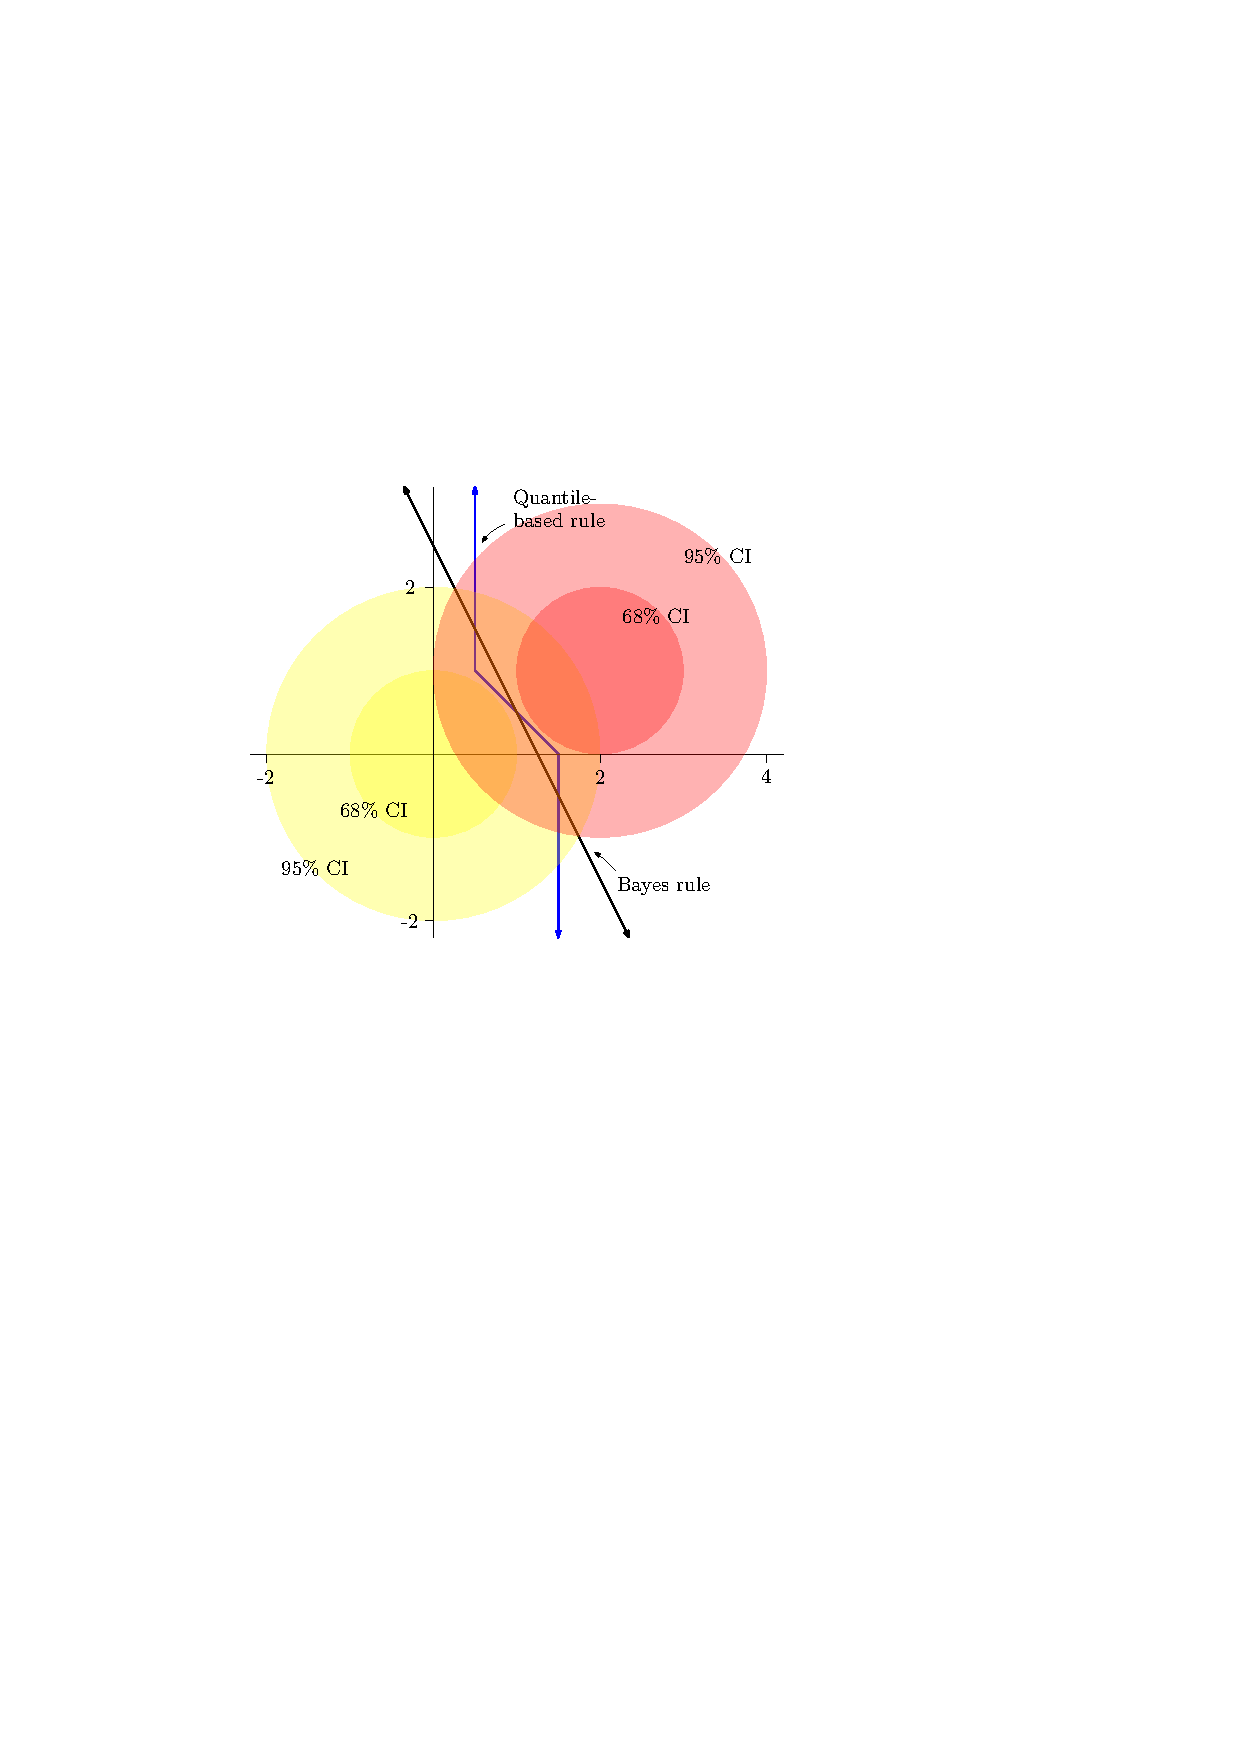
\includegraphics[width=0.96\textwidth]{gauss_ci}
  \end{minipage}
  \begin{minipage}[t]{0.44\linewidth}
    \flushright
    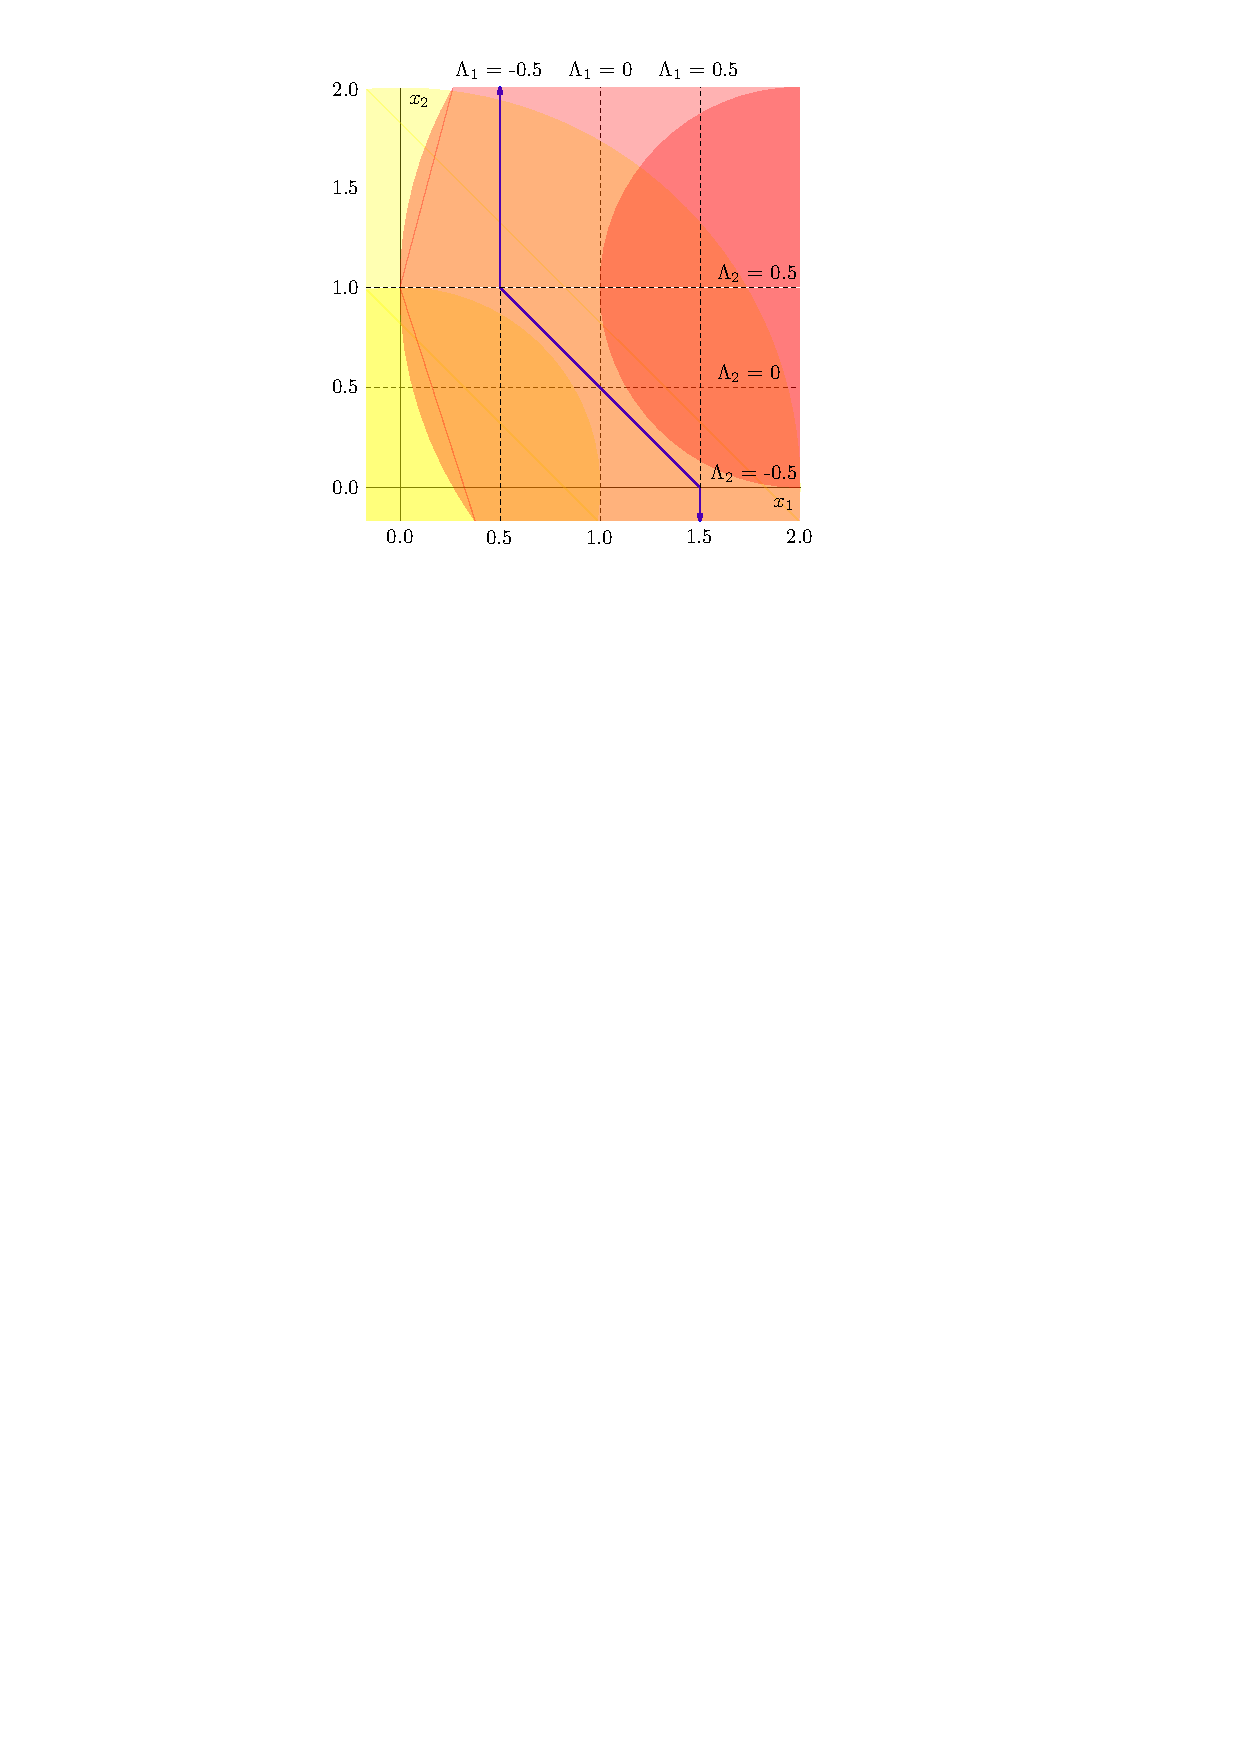
\includegraphics[width=1\textwidth]{gauss_quant_rule}
  \end{minipage}
\end{figure}

In a second example, shown as Figure \ref{fig:exponentiated-gaussian}, we
consider the setting of two location-shifted exponentiated Gaussian
distributions.  In more detail, if $(W_1, W_2) \sim N(\vec{0}, \vec{I})$, then
class 0 follows a distribution given by $(e^{W_1},\, e^{W_2})$ and class 1
follows a distribution given by $(e^{W_1} + 1,\, e^{W_2} + 1)$.  It turns out
that under this setting, the component-wise Bayes rule decision boundaries are
given by the location shift, which in this case is 1 for each component.  The
corresponding quantile level yields within-class quantiles of 0.5 and 1.5 for
the two classes for each component, so we obtain the decision boundary line
$\{(x_1, x_2) : x_2 = -x_1 + 2\}$ in the region $[0.5, 1.5]^2$.  Outside of this
region is a little bit more subtle.  The decision rule boundary lines shown in
Figure \ref{fig:exponentiated-gaussian} are contingent on the fact that we have
favorably chosen that tied distances be classified to the correct class
(i.e. the distribution with the yellow color).  Had we had chosen that the
tiebreaker had gone in the other direction then the decision rule boundary lines
outside of the region $[0.5, 1.5]^2$ would switch from going up and right to
left and down.  This unfavorable tiebreaker policy results in a 2.4\% decrease
in the composite quantile-based classifiers classification rate.  Otherwise the
classification rate for the composite quantile-based classifier is 0.71, while
the classification rate for the Bayes rule classifier is 0.75.

% This setting is
% interesting to consider because although this looks like a difficult case for
% quantile-based classifiers to handle, the classifier actually does really well
% in comparison to competitors in higher dimensions, as is shown in the numerical
% studies.

\begin{figure}[ht]
  \caption{Exponentiated Gaussian distributions classifier}
  \label{fig:exponentiated-gaussian}
  \centering
  \vspace{5mm}

  \begin{minipage}[t]{0.49\linewidth}
    \flushleft
    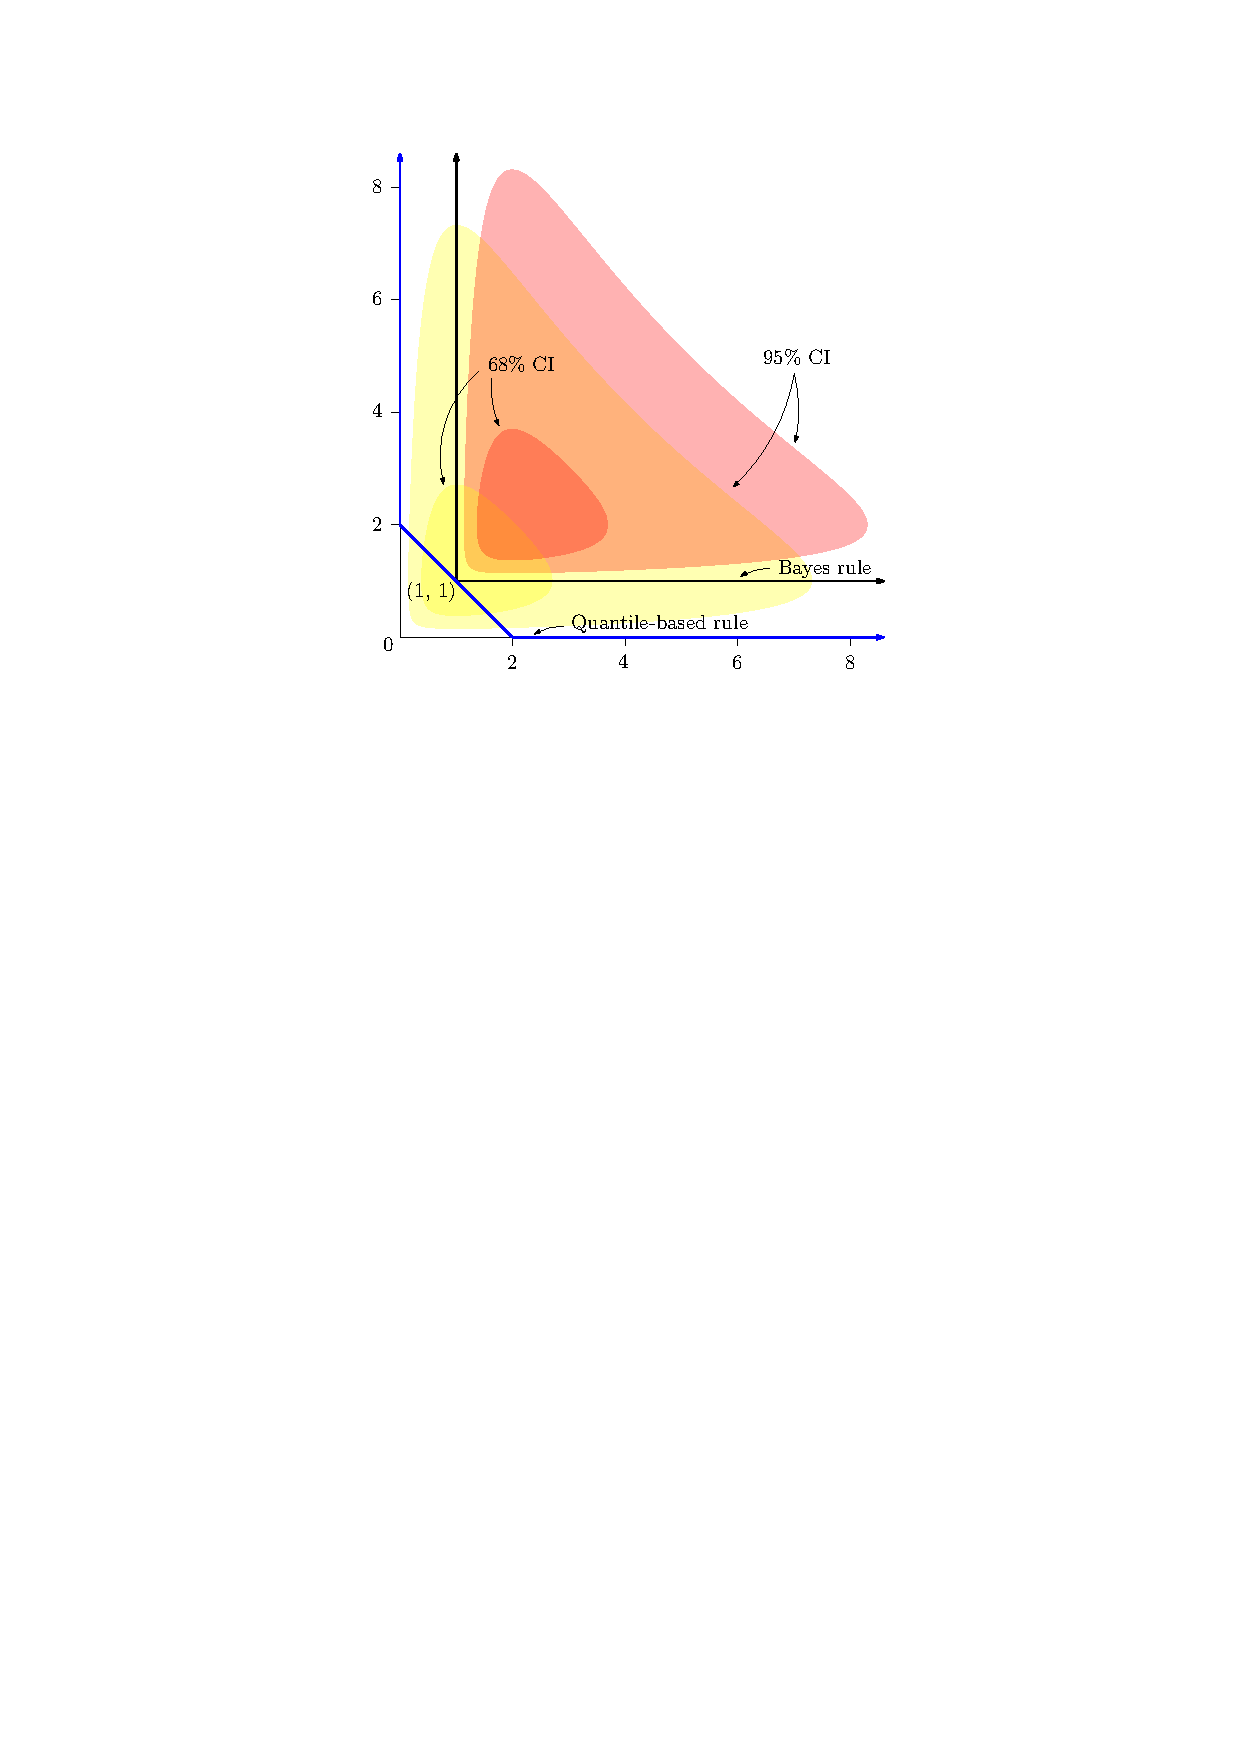
\includegraphics[width=0.95\textwidth]{exp_gauss_ci}
  \end{minipage}
  \begin{minipage}[t]{0.49\linewidth}
    \flushright
    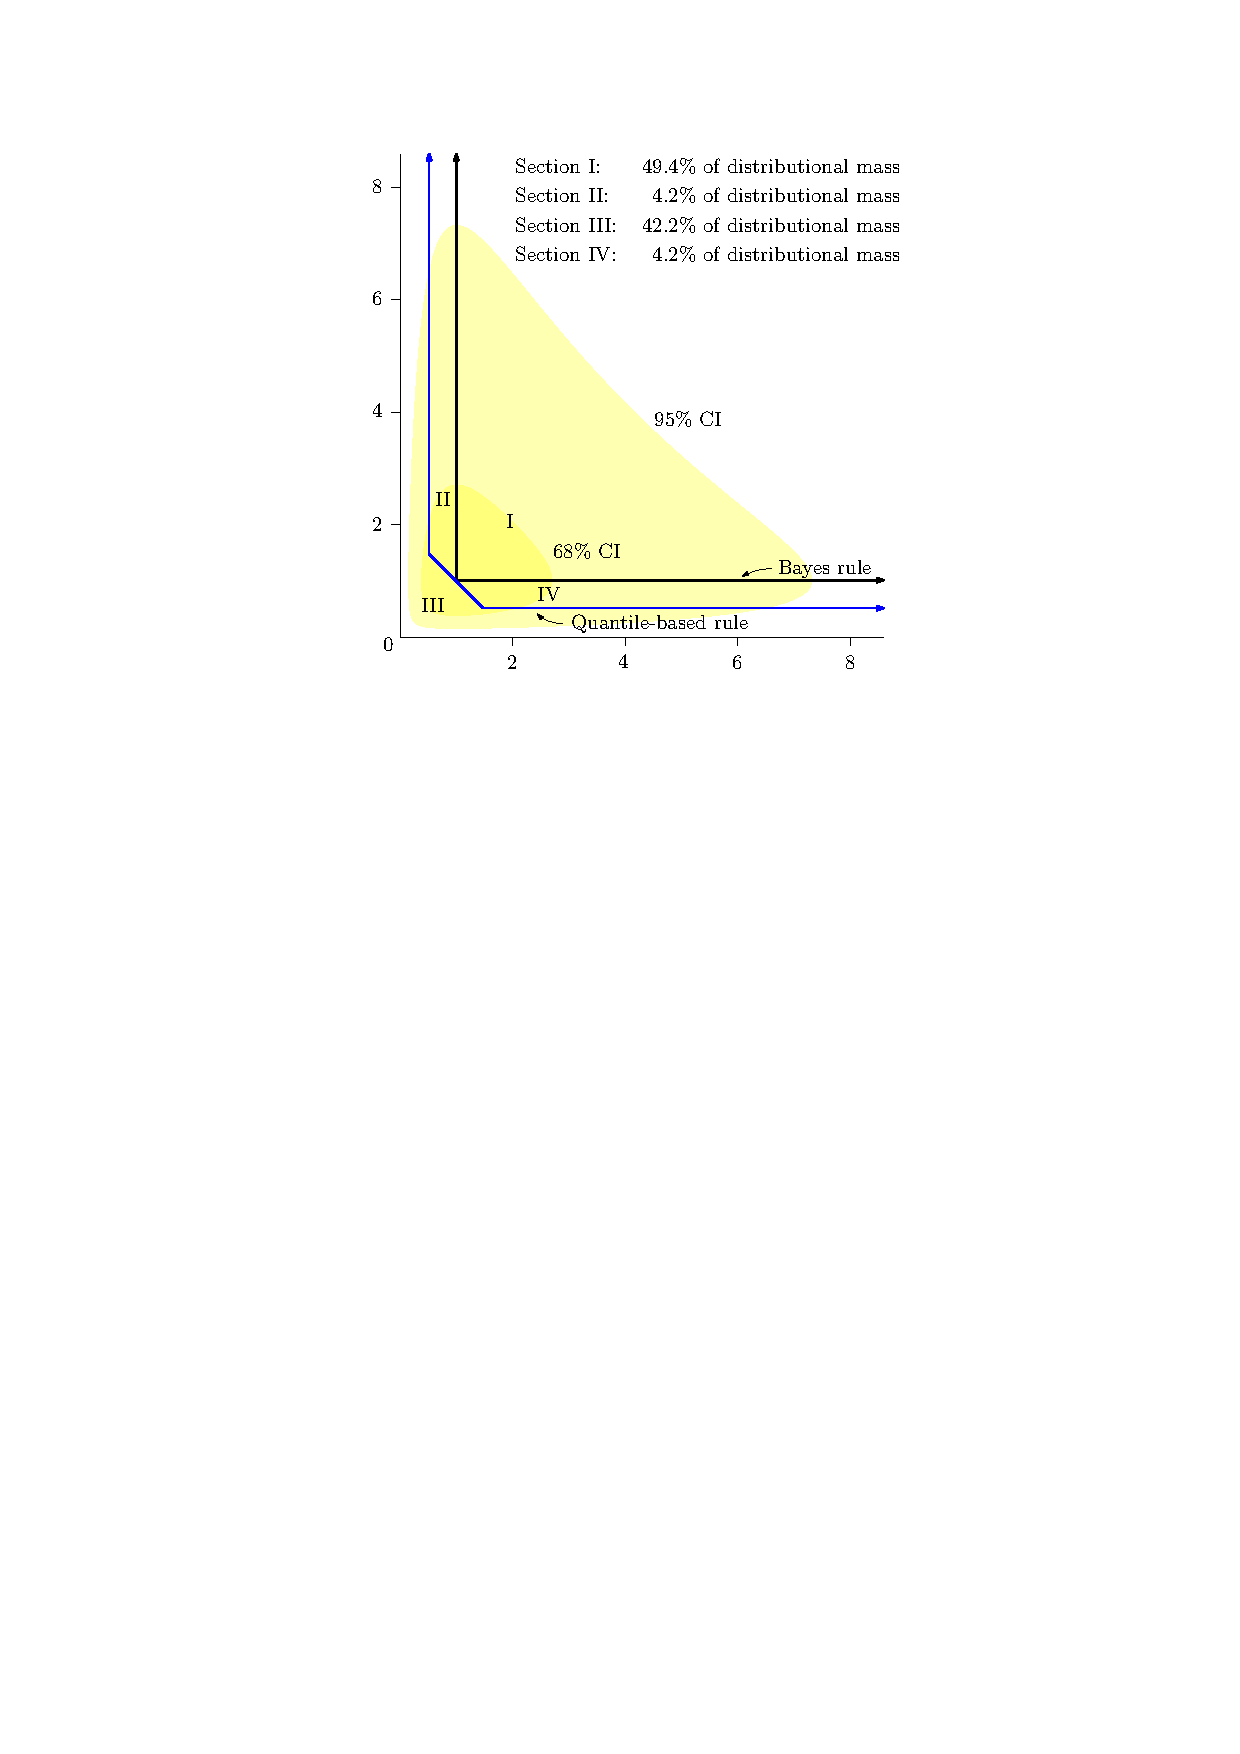
\includegraphics[width=0.95\textwidth]{exp_gauss_rule}
  \end{minipage}
\end{figure}



\subsubsection{Potential instabilities in quantile-based methods}
\label{sec:instabilities}

One potential instability of composite quantile-based classifiers is that the
direction of the decision rule boundary lines are dependent on the magnitude of
the difference between the component-wise class quantiles.  This causes raises
two concerns.  Firstly, changes in scale of the features can fundamentally
affect the classifier by changing which components are part of the linear
systems in the piecewise affine sets.  As a result, when some of the features in
the data are very different in scale to other features then we recommend some
sort of data transformations to try to keep the features at a similar scale
before performing classification.

On the other hand, a second potential source of instability for composite
quantile-based classifiers occurs when the magnitude of the differences between
the within-class quantiles is very similar for two or more features.  When this
is the case, small changes in the within-class quantile estimates can
fundamentally affect the classifier by changing which components are part of the
linear systems in the piecewise affine sets.  When the number of features is
small this can dramatically change the classifier; when the number of features
is larger, we expect such changes to have a diminished effect.  We also expect
averaging the model as discussed in Section \ref{sec:classifier-algorithm} to
help protect against this type of instability.


%%% Local Variables:
%%% mode: latex
%%% TeX-master: "cqc_paper"
%%% End:
